
% This LaTeX was auto-generated from MATLAB code.
% To make changes, update the MATLAB code and republish this document.

\documentclass{article}
\usepackage{graphicx}
\usepackage{color}

\sloppy
\definecolor{lightgray}{gray}{0.5}
\setlength{\parindent}{0pt}

\begin{document}

    
    

\section*{Final Problem 3 Simulation}

\begin{verbatim}
clear; close all; clc

X = random('Exponential', 1, [1e6,1]);
Y = random('Exponential', 1, [1e6,1]);
Z = random('Exponential', 1, [1e6,1]);

U = X./(X+Y);
V = (X+Y)./(X+Y+Z);
W = X+Y+Z;

w = 0:.01:30;
v = 0:.01:1;

pdV = fitdist(V,'Beta');
pdfV = pdf(pdV,v);

pdW = fitdist(W,'Gamma');
pdfW = pdf(pdW,w);

figure(1)
histogram(U,'Normalization','PDF');

figure(2)
hold on
histogram(V,'Normalization','PDF');
plot(v,pdfV,'LineWidth',2);
hold off

figure(3)
hold on
histogram(W,'Normalization','PDF');
plot(w,pdfW,'LineWidth',2);
hold off

%plot(pdU);
\end{verbatim}

\includegraphics [width=4in]{prob3_sim_01.eps}

\includegraphics [width=4in]{prob3_sim_02.eps}

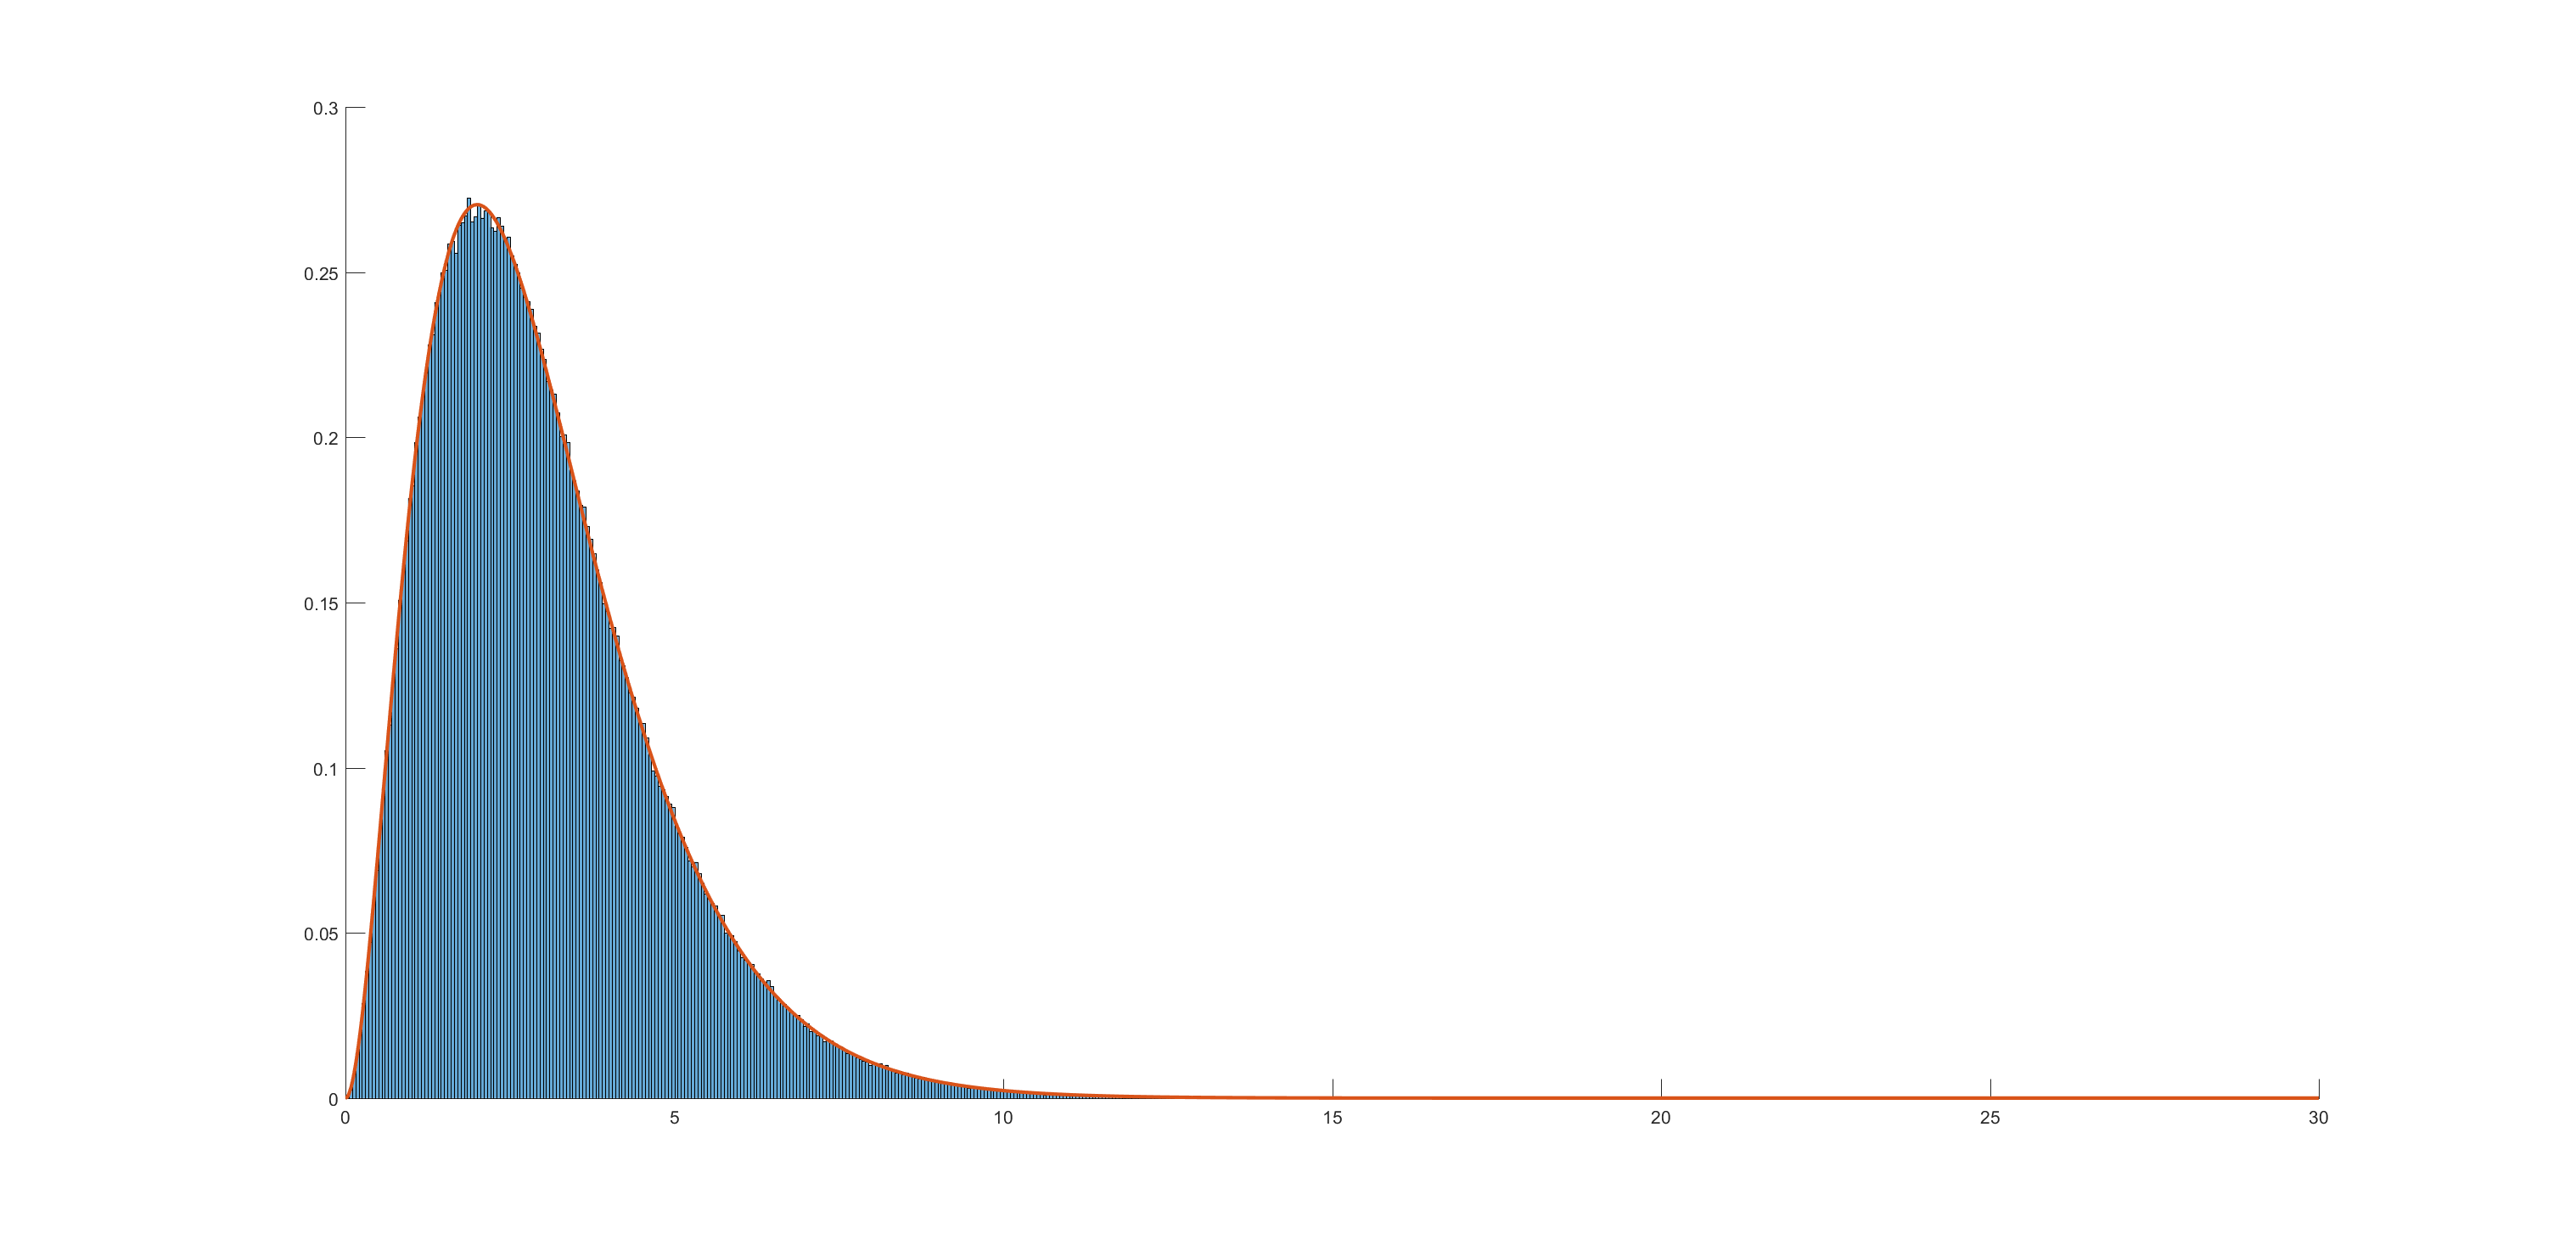
\includegraphics [width=4in]{prob3_sim_03.eps}



\end{document}
    
